\documentclass{article}
\usepackage{graphicx}

\title{2022 Summer Reading Challenge: Fermat’s Enigma}
\author{Jason Yao}

\begin{document}

\maketitle
A while ago, I was reading “Fermat’s Enigma”, by Simon Singh. Although two and a half decades old, I was still struck by the story behind the century-old problem. The book offered a glimpse into the concept of mathematical proof. A complete proof, much like mathematics as a whole, is like a house of cards, where the entire structure breaks down if one part does. Unlike the case in science, evidence is not enough. “Fermat’s enigma” details the four-hundred-year story behind Fermat’s last theorem, a small riddle posed by Fermat, who was known as the “prince of amateurs” among mathematicians. Although undoubtedly a great story, it was the concept of mathematical proof inside that interested me the most.

Proofs are generally agreed to have been used as early as ancient Greek times, and is acknowledged as one of the greatest achievements of Greek mathematicians, notably Euclid. Although they were mostly limited to geometry, he still revolutionized proofs in general. His book, “The Elements” lays the foundation for this, and as such is often regarded as the mathematical bible. Nowadays, proof theory treats proofs as inductively defined steps, and sometimes does not even require an assumption that axioms are true. This allows parallel theories as models of a concept to be considered, based on different sets of axioms. For example, non-Euclidean structures. However, the majority of mathematics is done with the general set of postulates.

 
A mathematical proof should be seamless from start to finish in order to be accepted. They are heavily dependent on previous theorems, and if a theorem is just slightly incorrect, every theorem that relies on it will also end up being unacceptable. Even evidence that a theorem works for every single number until the trillions, it is not proof that the theorem must be true.
\begin{center}
   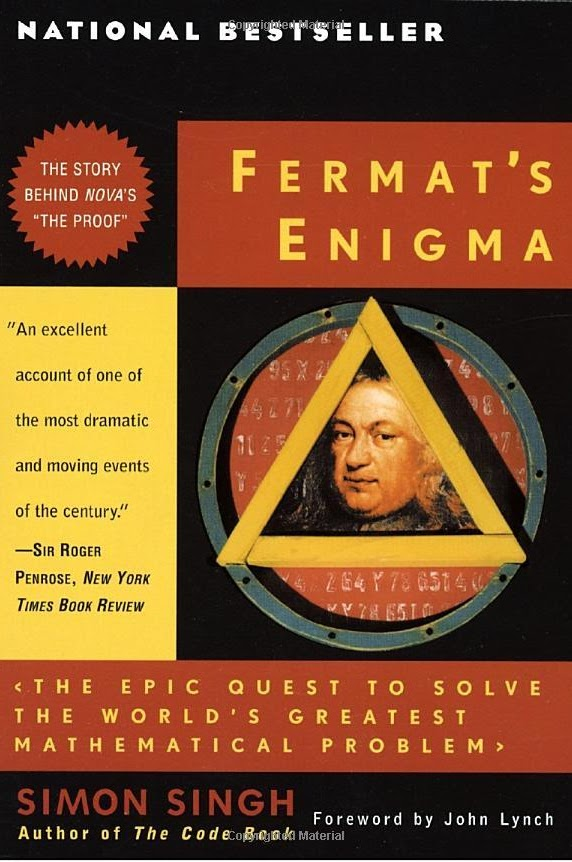
\includegraphics[scale=0.25]{Magazines/img/Vol1/fermats_enigma.jpg}
\end{center}
For example, a hypothesis by Leonard Euler, his Leonard of Powers Conjecture, is true for every number until 61917364224 (about 61 trillion). It could be worse however, for example, $n^{17}+9$ and $(n+1)^{17} + 9$ are relatively prime until $842443292559288932928819732230890$
$0672459420460792433$. There is no reason further conjectures are not as deceptive as either one of these. 

Mathematics is like the construction of an ever-growing structure made out of plywood. If one part rots or breaks, everything on top of it does too. Therefore, an acceptable proof is made out of irrefutable, logical, mathematical steps, which lead to a conclusion. The cornerstones are postulates, axioms, and definitions, things that are assumed to be true, and what things mean. For example, an example of a postulate is that for numbers $a$ and $b$, $a + b = b + a$. From these postulates, theorems, laws, and identities can be constructed, which can be used to construct more theorems, laws, and identities. A statement that is thought to be true but not proven so is known as a conjecture, or a hypothesis if frequently used as an assumption to create further progress if true. On a tangential sidenote, certain statements can be proven to be undecidable, which means that based on the accepted axioms, they cannot be proven to be true or false. 

Overall, a proof has a sacred meaning, it is the holy grail of math. Only a complete line of reasoning can be used in mainstream mathematics, because only they are acceptable. It is a rigorous and sometimes tedious process, but a necessary and almost romantic concept.
\end{multicols}
\end{document}